\begin{figure}[H]
    \centering
    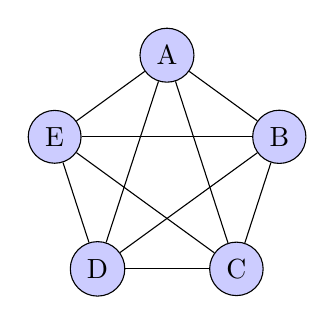
\begin{tikzpicture}
        \node[circle, draw, fill=blue!20] (A) at (90:1.5cm) {A};
        \node[circle, draw, fill=blue!20] (B) at (18:1.5cm) {B};
        \node[circle, draw, fill=blue!20] (C) at (-54:1.5cm) {C};
        \node[circle, draw, fill=blue!20] (D) at (234:1.5cm) {D};
        \node[circle, draw, fill=blue!20] (E) at (162:1.5cm) {E};
        \foreach \from/\to in {A/B, A/C, A/D, A/E, B/C, B/D, B/E, C/D, C/E, D/E}
            \draw (\from) -- (\to);
    \end{tikzpicture}
    \caption{Complete graph example.}
    \label{fig:complete-graph}
\end{figure}